%scritto da Federico Perin
\subsubsection{UCA 4 - Inserimento modalità di tracciamento}%kite level

\begin{figure}[h]
	\centering	
	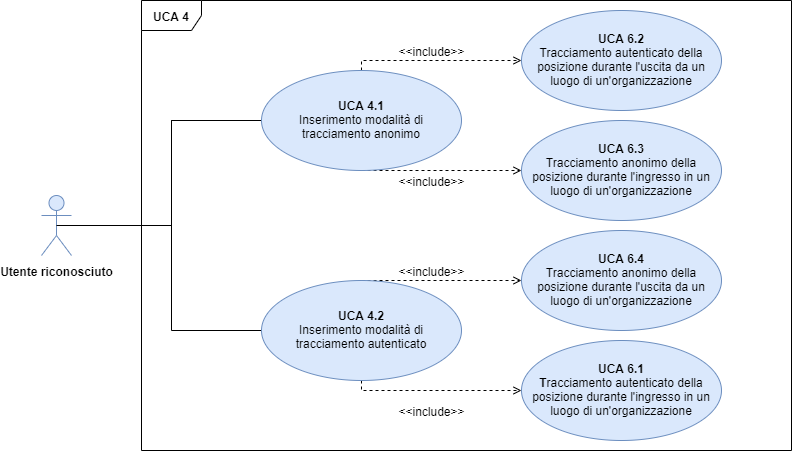
\includegraphics[scale=0.53]{sezioni/UseCase/Immagini/UCA4.png}
	\caption{UCA 4 - Inserimento modalità di tracciamento}
\end{figure}

\begin{itemize}
	\item \textbf{Attori primari:} Utente riconosciuto
	\item \textbf{Precondizione:} L'utente si è autenticato con le credenziali LDAP\ap{G} nella organizzazione\ap{G} in cui si trova e vuole selezionare la modalità di tracciamento\ap{G}.
	\item \textbf{Postcondizione:} L'utente viene tracciato secondo la modalità da lui scelta precedentemente.
	\item \textbf{Scenario principale:} L'utente accede alla funzionalità di selezione della modalità di tracciamento.
	\item \textbf{Flusso di eventi:}
	\begin{enumerate}
		\item L'utente accede alla funzione di inserimento modalità di tracciamento;
		\item L'utente può scegliere la modalità di tracciamento anonimo\ap{G} [UCA 4.1] oppure la modalità di tracciamento autenticato\ap{G} [UCA 4.2].
	\end{enumerate}
\end{itemize}

\subsubsection{UCA 4.1 - Inserimento modalità di tracciamento anonimo}%sea level
\begin{itemize}
\item \textbf{Attori primari:} Utente riconosciuto
\item \textbf{Precondizione:} L'utente si è autenticato con le credenziali LDAP\ap{G} nella organizzazione\ap{G} in cui si trova e vuole selezionare la modalità di tracciamento anonimo\ap{G}].
\item \textbf{Postcondizione:} L'utente viene tracciato secondo la modalità anonimo\ap{G}.
\item \textbf{Scenario principale:} L'utente accede alla funzionalità inserimento modalità di tracciamento\ap{G} e inserisce la modalità anonimo\ap{G}.
\item \textbf{Flusso di eventi:}
\begin{enumerate}
	\item L'utente accede alla funzione di inserimento modalità di tracciamento anonimo\ap{G};
	\item L'utente inserisce la modalità di tracciamento anonimo\ap{G}.
\end{enumerate}

\end{itemize}

\subsubsection{UCA 4.2 - Inserimento modalità di tracciamento autenticato}%sea level
\begin{itemize}
	\item \textbf{Attori primari:} Utente riconosciuto
	\item \textbf{Precondizione:} L'utente si è autenticato con le credenziali LDAP\ap{G} nella organizzazione in cui si trova e vuole selezionare la modalità di tracciamento autenticato\ap{G}.
	\item \textbf{Postcondizione:} L'utente viene tracciato secondo la modalità autenticato\ap{G}.
	\item \textbf{Scenario principale:} L'utente accede alla funzionalità inserimento modalità di tracciamento\ap{G} e inserisce la modalità autenticato\ap{G}.
	\begin{enumerate}
		\item L'utente accede alla funzione di inserimento modalità di tracciamento autenticato\ap{G};
		\item L'utente inserisce la modalità di tracciamento autenticato\ap{G}.
	\end{enumerate}
\end{itemize}
